\begin{frame}{Parametric Curves}
\begin{center}
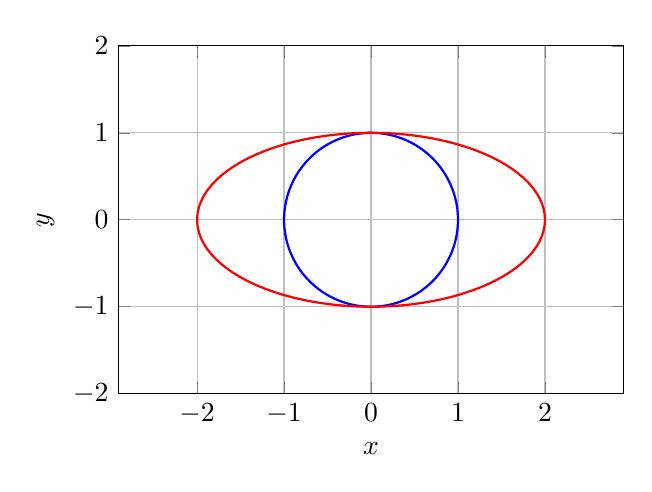
\begin{tikzpicture}
\begin{axis}[
    xlabel={$x$},
    ylabel={$y$},
    grid=both,
    xmin=-2, xmax=2,
    ymin=-2, ymax=2,
    width=8cm,
    height=6cm,
    axis equal
]
\addplot[thick, blue, domain=0:2*pi, samples=100] ({cos(deg(x))}, {sin(deg(x))});
\addplot[thick, red, domain=0:2*pi, samples=100] ({2*cos(deg(x))}, {sin(deg(x))});
\end{axis}
\end{tikzpicture}
\end{center}

\footnotesize
\texttt{\textbackslash addplot[thick, blue] (\{cos(deg(x))\}, \{sin(deg(x))\})}
\end{frame}